\documentclass{beamer}

\usepackage[utf8]{inputenc}

\usetheme{Warsaw}


\title{Maxwell Equations}
\author{listenzcc}
\institute[VFU] % (optional)
{
  \inst{1}%
  Faculty of Physics\\
  Very Famous University
  \and
  \inst{2}%
  Faculty of Chemistry\\
  Very Famous University
}

\date{\today}

\begin{document}

\frame{\titlepage}

\begin{frame}
    \frametitle{Table of Contents}
    \tableofcontents
\end{frame}


\section{Prepare Knowledge}
\AtBeginSection[]
{
    \begin{frame}
        \frametitle{Table of Contents}
        \tableofcontents[currentsection]
    \end{frame}
}

\begin{frame}
    \frametitle{Scalar and vector field}
    A function of space is known as a field.
    Let an arbitrary 3-D coordinate system be given.

    \begin{block}{Scalar field}
        If to each position $x = (x_{1}, x_{2}, x_{3})$ of a region in space, it corresponds a scalar $\phi (x_{1}, x_{2}, x_{3})$, then $\phi$ is called a \emph{scalar field}.

        Like \emph{density} field.
    \end{block}

    \begin{block}{Vector field}
        If to each position $x = (x_{1}, x_{2}, x_{3})$ of a region in space, it corresponds a vector $\vec{a} (x_{1}, x_{2}, x_{3})$, then $\vec{a}$ is called a \emph{vector field}.

        Like \emph{velocity} field.
    \end{block}

    \pause
    How does scalar or vector field change along spatial dimensions?
\end{frame}

\begin{frame}
    \frametitle{Scalar and vector field}
    An example
    \begin{figure}[H]
        \centering
        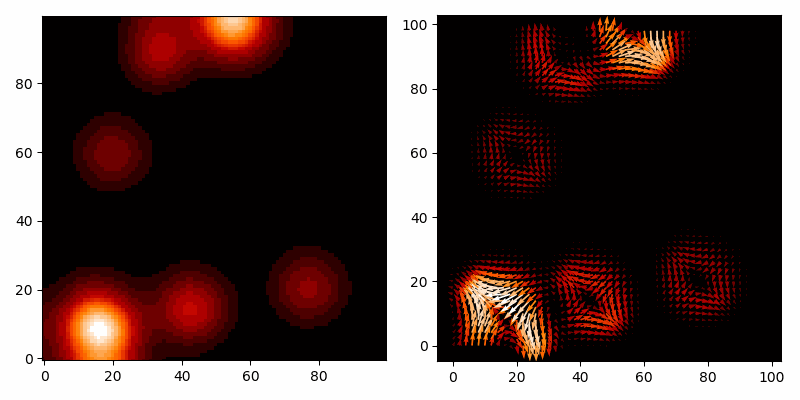
\includegraphics[height=0.5\textheight]{heatmap.png}
        \caption{Heat Map}
        \label{fig: Heat map}
    \end{figure}
\end{frame}

\begin{frame}
    \frametitle{Nabla operator $\nabla$}
    Partial derivatives is an useful tool to measure the changes along spatial dimensions.

    For scalar field
    \begin{equation}
        \partial_{i} \phi = \frac{\partial}{\partial x_{i}} \phi
    \end{equation}

    For vector field
    \begin{equation}
        (\partial_{i} \vec{a}) (\vec{r}) = \lim_{\Delta x_{i} \rightarrow 0} \frac{\vec{a}(\vec{r} + \Delta x_{i} \vec{e}_{i}) - \vec{a}(\vec{r})}{\Delta x_{i}}
    \end{equation}

    To simplify the partial derivatives, we imply \emph{Nabla operator}.
    \begin{alertblock}{Nabla operator}
        \begin{equation}
            \nabla (\cdot) = \sum_{i} \vec{e}_{i} \partial_{i} (\cdot)
        \end{equation}
    \end{alertblock}

\end{frame}

\begin{frame}
    \frametitle{Gradient, diverence, curl}

    \begin{block}{Gradient}
        \begin{equation}
            grad \phi = \nabla \phi = \sum_{i} \vec{e}_{i} \partial_{i} \phi
        \end{equation}
    \end{block}

    \begin{block}{Divergence}
        \begin{equation}
            div \vec{a} = \nabla \vec{a} = \sum_{i} \partial_{i} \vec{a}
        \end{equation}
    \end{block}

    \begin{block}{Curl}
        \begin{equation}
            curl \vec{a} = \nabla \times \vec{a} = det
            \begin{pmatrix}
                \vec{e}_{1}  & \vec{e}_{1}  & \vec{e}_{1}  \\
                \partial_{1} & \partial_{1} & \partial_{1} \\
                \vec{a}_{1}  & \vec{a}_{1}  & \vec{a}_{1}
            \end{pmatrix}
        \end{equation}
    \end{block}

\end{frame}

\section{Maxwell Equations}
\AtBeginSection[]
{
    \begin{frame}
        \frametitle{Table of Contents}
        \tableofcontents[currentsection]
    \end{frame}
}

\begin{frame}
    \frametitle{Definition}
    Maxwell Equations describe the dynamic of Electromagnetic Wave.
    \begin{columns}

        \column{0.5\textwidth}
        \begin{equation}
            \nabla \cdot \vec{D} = \rho
        \end{equation}
        \begin{equation}
            \nabla \cdot \vec{B} = 0
        \end{equation}
        \begin{equation}
            \nabla \times \vec{E} = - \frac{\partial{\vec{B}}}{\partial{t}}
        \end{equation}
        \begin{equation}
            \nabla \times \vec{H} = \frac{\partial{\vec{D}}}{\partial{t}} + \vec{J}
        \end{equation}

        \column{0.5\textwidth}
        \begin{table}[h]
            \centering
            \caption{Meaning}
            \begin{tabular}{|c|l|}
                \hline
                $\vec{D}$ & Electric Flux Density   \\\hline
                $\vec{B}$ & Magnetic Flux Density   \\\hline
                $\vec{E}$ & Electric Field          \\\hline
                $\vec{H}$ & Magnetic Field          \\\hline
                $\vec{J}$ & Current Density         \\\hline
                $\rho$    & Electric Charge Density \\
                \hline
            \end{tabular}
        \end{table}

    \end{columns}

    \vspace{5mm}
    where $\vec{B} = \mu \vec{H}$, $\vec{D} = \epsilon \vec{E}$.
\end{frame}

\begin{frame}
    \frametitle{Example}
    In vacuum space, the Maxwell Equations are re-written as
    \begin{equation}
        \nabla \cdot \vec{E} = 0
    \end{equation}
    \begin{equation}
        \nabla \times \vec{E} = - \frac{\partial{\vec{B}}}{\partial{t}}
    \end{equation}
    \begin{equation}
        \nabla \cdot \vec{B} = 0
    \end{equation}
    \begin{equation}
        \nabla \times \vec{B} = \mu_{0} \epsilon_{0} \frac{\partial{\vec{E}}}{\partial{t}}
    \end{equation}
\end{frame}

\begin{frame}
    \frametitle{Example}
    $\vec{E}$ and $\vec{B}$ is almost symmetry.
    \begin{equation}
        \nabla \times (\nabla \times \vec{E}) =
        - \mu_{0} \epsilon_{0} \frac{\partial^{2}}{\partial{t^{2}}} \vec{E}
    \end{equation}
    \begin{equation}
        \nabla \times (\nabla \times \vec{B}) = - \mu_{0} \epsilon_{0} \frac{\partial^{2}}{\partial{t^{2}}} \vec{B}
    \end{equation}
    use
    \begin{equation}
        \nabla \times (\nabla \times \vec{X}) =
        \nabla \cdot (\nabla \cdot \vec{X}) - \nabla^{2} \vec{X}
    \end{equation}
    we have
    \begin{equation}
        \nabla^{2} \vec{X} = \mu_{0} \epsilon_{0} \frac{\partial^{2}}{\partial{t^{2}}} \vec{X}
    \end{equation}
    Solve the wave function, the wave speed is $c=\frac{1}{\sqrt{\mu_{0} \epsilon_{0}}}$.\footnote{$\mu_{0}=8. 854187817 \times 10^{-12} F/m$, $\epsilon_{0}=4 \pi \times 10^{-7} N/A^{2}$}
\end{frame}

\section{Forward and Backward Process}

\begin{frame}
    \frametitle{Forward process}
    \begin{columns}
        \column{0.5\textwidth}
        Volume conductor
        \begin{itemize}
            \item Scalp
            \item Skull
            \item CSF
            \item Grey matter
            \item White matter
            \item Air pockets
            \item Conductivity tensor
        \end{itemize}

        \column{0.5\textwidth}
        \begin{figure}[H]
            \centering
            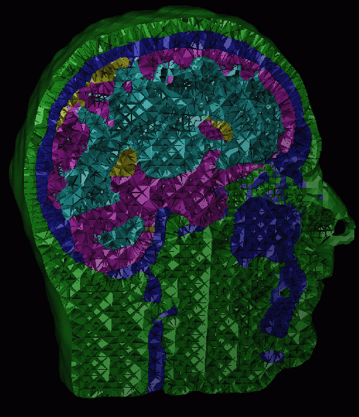
\includegraphics[height=0.5\textheight]{skull.png}
            \caption{Skull}
            \label{fig:Skull}
        \end{figure}

    \end{columns}
\end{frame}

\begin{frame}
    \frametitle{Forward process}
    \begin{columns}
        \column{0.5\textwidth}
        Source model
        \begin{itemize}
            \item Neurons – brain cells, building blocks
            \item Pyramidal cells $10^{-5} per mm$ in cortex
            \item Send electric impulse (action potential $~20fA$ per synapse)
            \item $40 mm^{2}$ of active cortex
            \item Current $I_{0} = 10 nA$
            \item Source  decays  $d = 0.1 mm$
            \item Current dipole $P = I0 * d$
        \end{itemize}

        \column{0.5\textwidth}
        \begin{figure}[H]
            \centering
            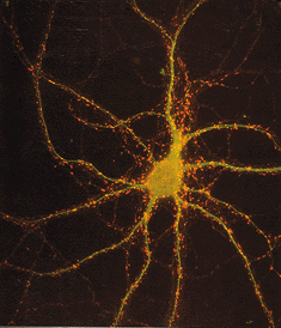
\includegraphics[height=0.5\textheight]{source_model.png}
            \caption{Source model}
            \label{fig:Source model}
        \end{figure}

    \end{columns}
\end{frame}

\begin{frame}
    \frametitle{Forward process}
    \begin{columns}
        \column{0.5\textwidth}
        Physical model
        \begin{itemize}
            \item Head is a volume conductor
            \item Concentrated current source (intra-cellular currents)
            \item Passive return volume currents (extra-cellular currents)
                  \begin{equation*}
                      \vec{J} = \vec{J_{i}} + \vec{J_{e}}
                  \end{equation*}
            \item No flux boundary conditions
                  \begin{equation*}
                      (\vec{J_{1}} - \vec{J_{2}}) \cdot \vec{n} = 0
                  \end{equation*}
        \end{itemize}

        \column{0.5\textwidth}
        \begin{figure}[H]
            \centering
            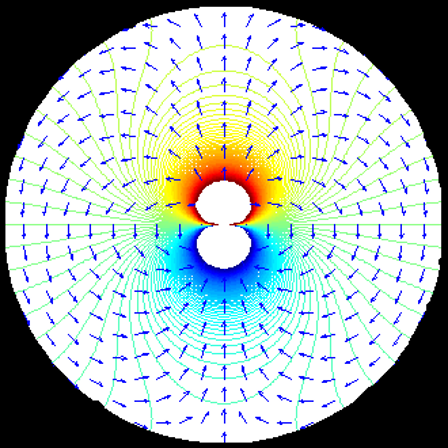
\includegraphics[height=0.5\textheight]{physical_model.png}
            \caption{Physical model}
            \label{fig: Physical model}
        \end{figure}

    \end{columns}
\end{frame}

\begin{frame}
    \frametitle{Forward process}
    Forward problem solution
    \begin{columns}
        \column{0.5\textwidth}
        \begin{itemize}
            \item Estimate the potential on the skull surface
            \item Knowing the currents beneath the skull
        \end{itemize}

        \column{0.5\textwidth}
        \begin{figure}[H]
            \centering
            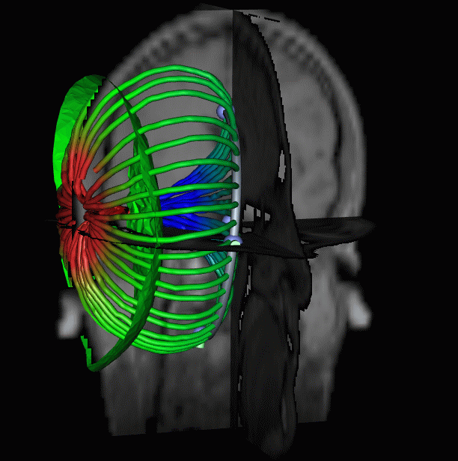
\includegraphics[height=0.5\textheight]{forward_solution.png}
            \caption{Forward solution}
            \label{fig: Forward solution}
        \end{figure}

    \end{columns}
\end{frame}

\begin{frame}
    \frametitle{Mathematical model}
    Poisson equation
    \begin{equation}
        \nabla \cdot (\sigma \nabla \Phi) = \sum \vec{I_{s}}, \vec{I_{s}} in \Omega
    \end{equation}
    Neumann boundary conditions
    \begin{equation}
        \sigma (\nabla \Phi) \cdot n = 0
    \end{equation}
    Dipole current source
    \begin{equation}
        I_{s}(\vec{r}) = \lim_{d \rightarrow 0} \vec{I_{0}}
        ( \delta (\vec{r} - \vec{r_{s}} - \frac{d}{2}) - \delta (\vec{r} - \vec{r_{s}} + \frac{d}{2}) )
    \end{equation}
\end{frame}

\begin{frame}
    \frametitle{Forward estimation}
    The forward solution is exampled as following
    \begin{figure}[H]
        \centering
        \includegraphics[height=0.5\textheight]{Forward_estimation.png}
        \caption{Forward estimation}
        \label{fig: Forward estimation}
    \end{figure}
\end{frame}

\begin{frame}
    \frametitle{Backward process}
    The reverse process of forward process is Backward process.

    EEG measures the potential on the skull surface
    \begin{columns}
        \column{0.5\textwidth}
        \begin{figure}[H]
            \centering
            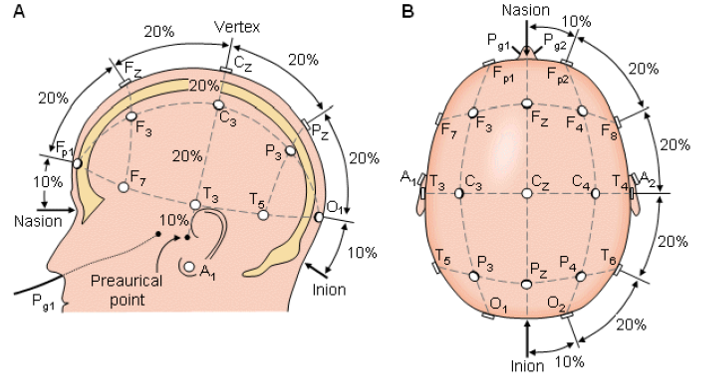
\includegraphics[height=0.4\textheight]{EEG_hat.png}
            \caption{EEG hat}
            \label{fig: EEG hat}
        \end{figure}

        \column{0.5\textwidth}
        \begin{figure}[H]
            \centering
            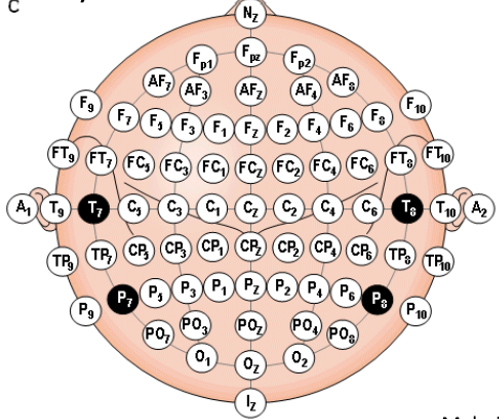
\includegraphics[height=0.4\textheight]{EEG_layout.png}
            \caption{EEG layout}
            \label{fig: EEG layout}
        \end{figure}
    \end{columns}
\end{frame}

\section{Source Location}

\begin{frame}
    \frametitle{Formulation}
\end{frame}

\begin{frame}
    \frametitle{Solution}
\end{frame}

\section{Slide Samples}

\begin{frame}
    \frametitle{Items}
    \begin{itemize}
        \item<1-> Text visible on slide 1
        \item<2-> Text visible on slide 2
        \item<3> Text visible on slide 3
        \item<4-> Text visible on slide 4
    \end{itemize}
\end{frame}

\begin{frame}
    \frametitle{Pause}
    In this slide \pause
    the text will be partially visible \pause
    And finally everything will be there
\end{frame}

\begin{frame}
    \frametitle{Sample frame title}

    In this slide, some important text will be
    \alert{highlighted} because it's important.
    Please, don't abuse it.

    \begin{block}{Remark}
        Sample text
    \end{block}

    \begin{alertblock}{Important theorem}
        Sample text in red box
    \end{alertblock}

    \begin{examples}
        Sample text in green box. The title of the block is ``Examples".
    \end{examples}
\end{frame}

\begin{frame}
    \frametitle{Two-column slide}

    \begin{columns}

        \column{0.5\textwidth}
        This is a text in first column.
        $$E=mc^2$$
        \begin{itemize}
            \item First item
            \item Second item
        \end{itemize}

        \column{0.5\textwidth}
        This text will be in the second column
        and on a second through this is a nice looking
        layout in some cases.

    \end{columns}
\end{frame}

\end{document}